


\begin{frame}{Sparse Matrix-Matrix Multiplications}

 \begin{block}{Sequential MatMatMult in PETSc}
  \begin{itemize}
   \item Sorted
   \item Scalable
   \item Scalable, fast
   \item Heap
   \item BTHeap
   \item Linked-list condensed
   \item RowMerge -- {\color{red}NEW!}
   \item RowMerge2 -- {\color{red}NEW!}
  \end{itemize}
 \end{block}

 \pause
 \begin{block}{Two Stages}
  \begin{itemize}
   \item Symbolic phase: Determine sparsity pattern
   \item Numeric phase: Compute numerical values, sparsity pattern known
  \end{itemize}
 \end{block}

\end{frame}




\begin{frame}{Sparse Matrix-Matrix Multiplications}

 \begin{center}\Large \textbf{Good News:} \\[2em] %\includegraphics[width=0.6\textwidth]{figures/good-news}\\ {\tiny http://www.dsoconnections.org/wp-content/uploads/2017/05/Good-news-750x400.jpg}\\[2em]
                      \textbf{Numeric phase is easy!}\end{center}

\end{frame}


\begin{frame}{Sparse Matrix-Matrix Multiplications}

\begin{center}
\only<1>{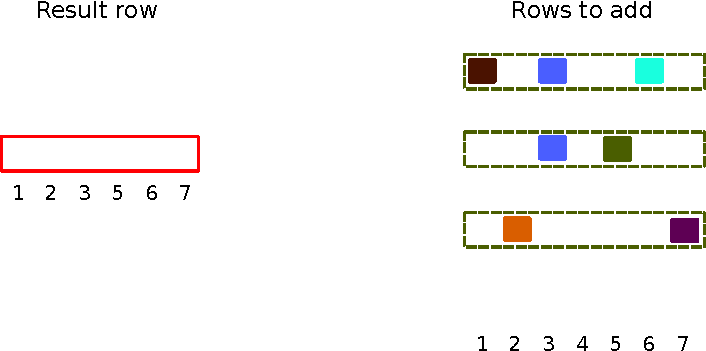
\includegraphics[width=0.7\textwidth]{figures/spgemm-numeric-1} }\only<2>{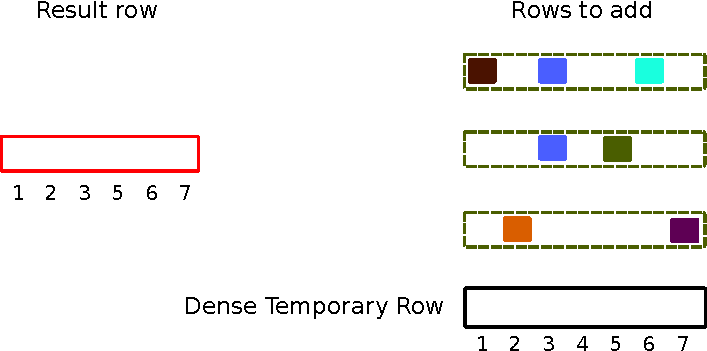
\includegraphics[width=0.7\textwidth]{figures/spgemm-numeric-2} }\only<3>{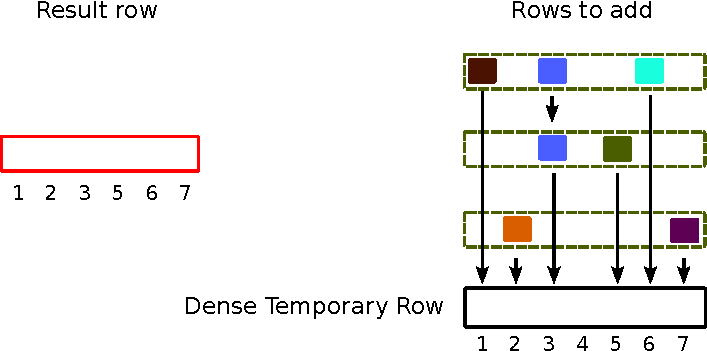
\includegraphics[width=0.7\textwidth]{figures/spgemm-numeric-3} }\only<4>{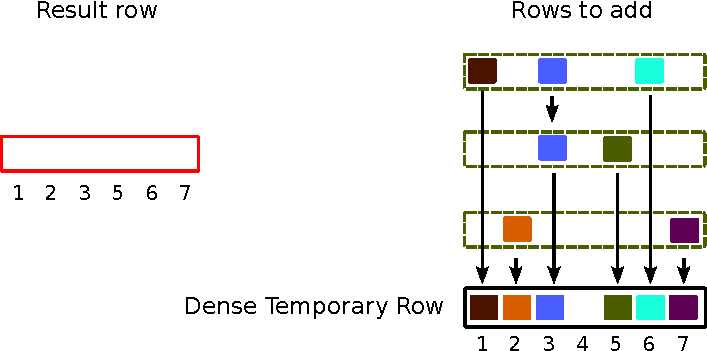
\includegraphics[width=0.7\textwidth]{figures/spgemm-numeric-4} }\only<5>{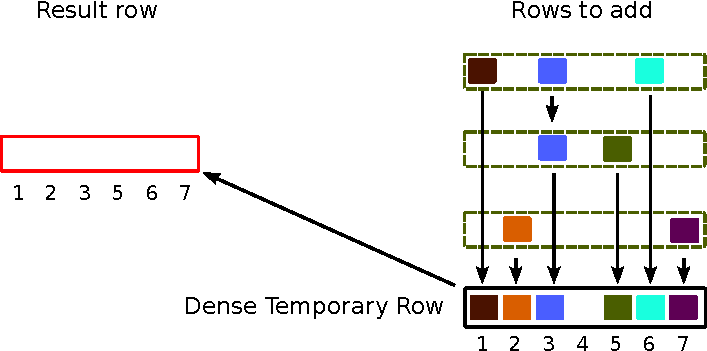
\includegraphics[width=0.7\textwidth]{figures/spgemm-numeric-5} }\only<6->{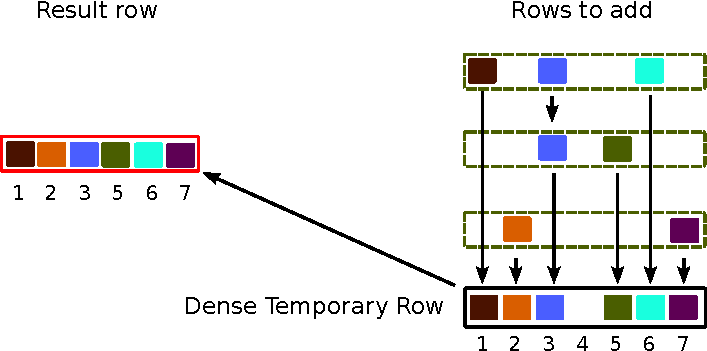
\includegraphics[width=0.7\textwidth]{figures/spgemm-numeric-6} }
\end{center}


 \begin{block}{Numeric Phase}
  \begin{itemize}
   \visible<2->{\item Merge directly to dense array}
   \visible<5->{\item Pick up nonzeros to form $\mathbf{C}$}
  \end{itemize}
 \end{block}

\end{frame}




\begin{frame}{Sparse Matrix-Matrix Multiplications}

 \begin{center}\Large \textbf{Bad News:} \\[2em] %\includegraphics[width=0.5\textwidth]{figures/bad-news}\\ {\tiny http://workingcapitalreview.com/wp-content/uploads/2015/03/20120802221109\_badnews.jpg}\\[2em]
                      \textbf{Symbolic phase is tricky!}\end{center}

\end{frame}





\begin{frame}{Sparse Matrix-Matrix Multiplications}

\begin{center}
\only<1>{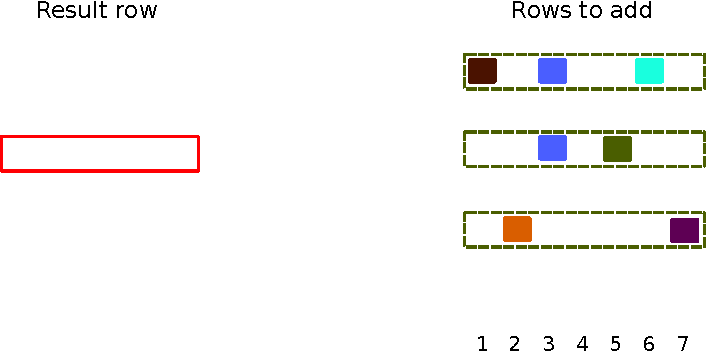
\includegraphics[width=0.7\textwidth]{figures/spgemm-sorted-1} }\only<2>{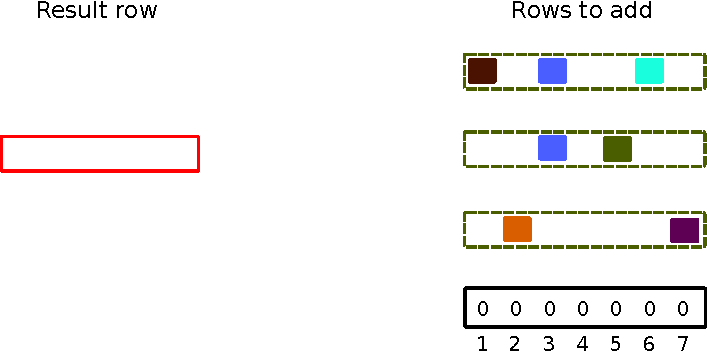
\includegraphics[width=0.7\textwidth]{figures/spgemm-sorted-2} }\only<3>{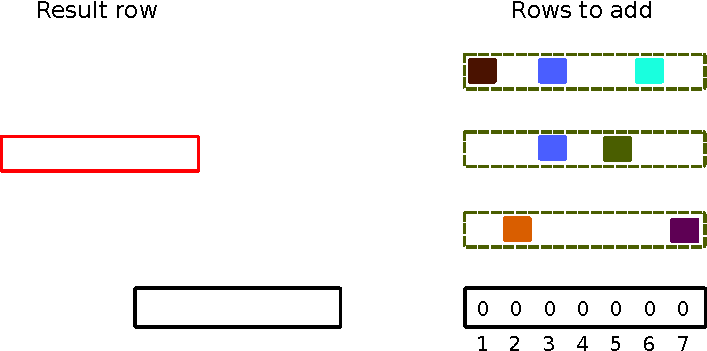
\includegraphics[width=0.7\textwidth]{figures/spgemm-sorted-3} }\only<4>{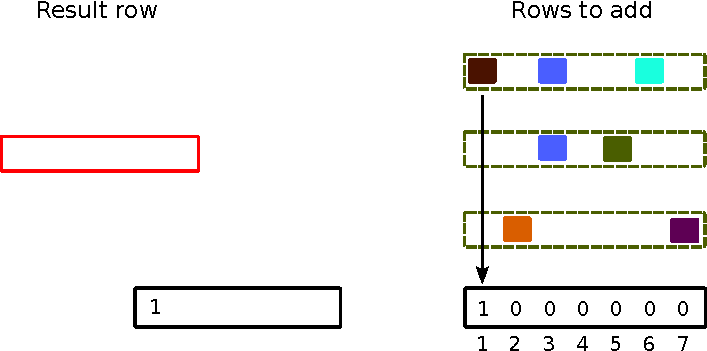
\includegraphics[width=0.7\textwidth]{figures/spgemm-sorted-4} }\only<5>{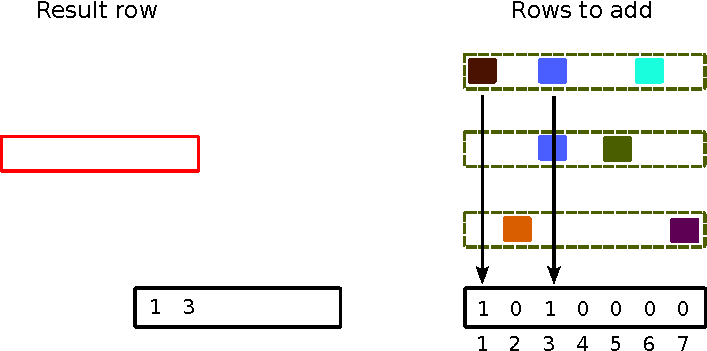
\includegraphics[width=0.7\textwidth]{figures/spgemm-sorted-5} }\only<6>{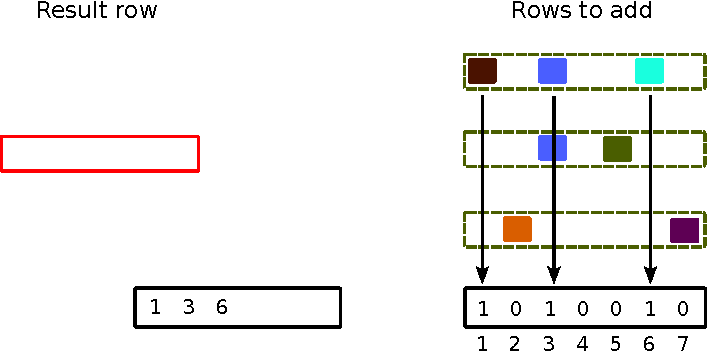
\includegraphics[width=0.7\textwidth]{figures/spgemm-sorted-6} }\only<7>{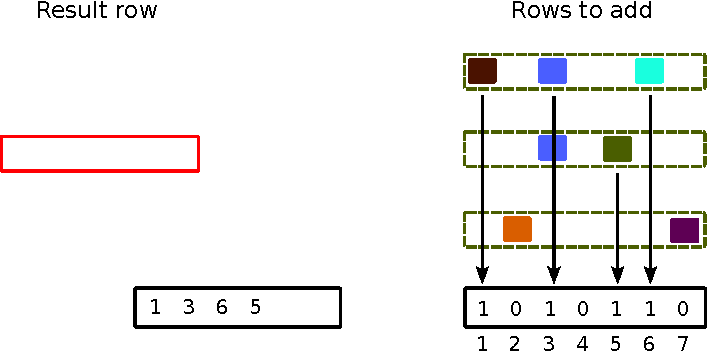
\includegraphics[width=0.7\textwidth]{figures/spgemm-sorted-7} }\only<8>{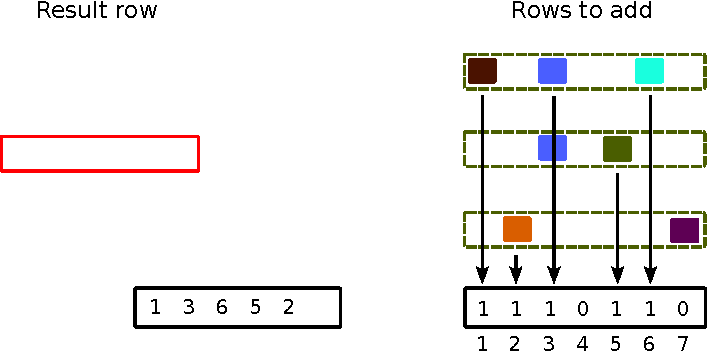
\includegraphics[width=0.7\textwidth]{figures/spgemm-sorted-8} }\only<9>{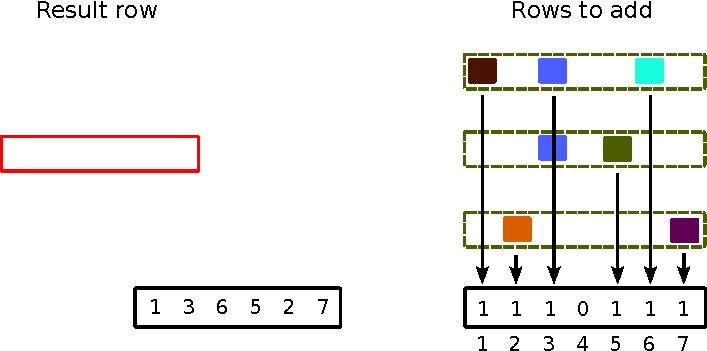
\includegraphics[width=0.7\textwidth]{figures/spgemm-sorted-9} }\only<10>{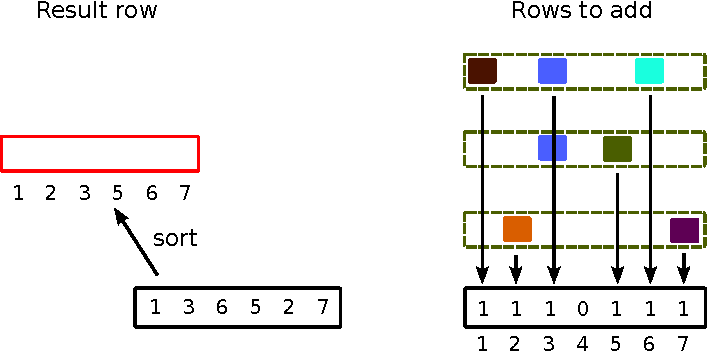
\includegraphics[width=0.7\textwidth]{figures/spgemm-sorted-10} }
\end{center}

 \begin{block}{Sorted MatMatMult in PETSc}
  \begin{itemize}
   \item Dense flag array
   \item Segmented buffer for nonzero indices
  \end{itemize}
 \end{block}

\end{frame}


\begin{frame}{Sparse Matrix-Matrix Multiplications}

\begin{center}
\only<1>{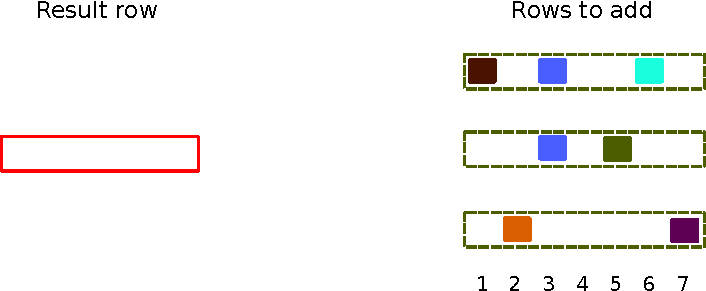
\includegraphics[width=0.7\textwidth]{figures/spgemm-scalable-2} }\only<2>{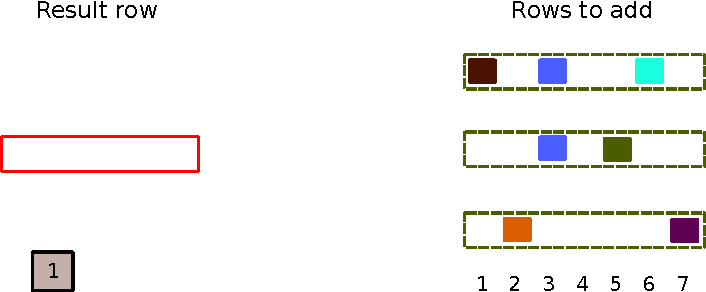
\includegraphics[width=0.7\textwidth]{figures/spgemm-scalable-3} }\only<3>{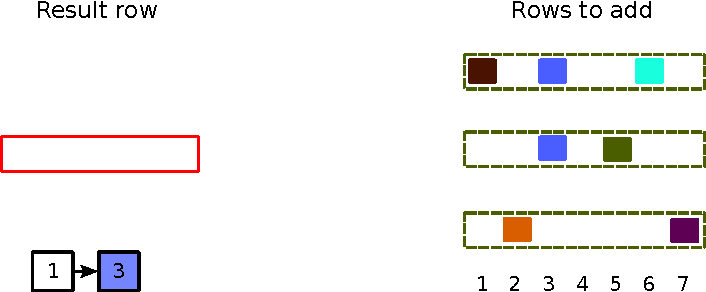
\includegraphics[width=0.7\textwidth]{figures/spgemm-scalable-4} }\only<4>{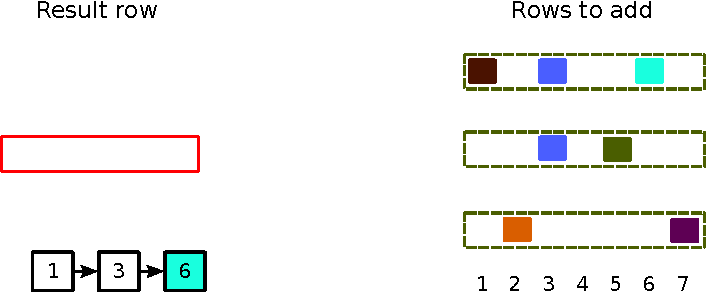
\includegraphics[width=0.7\textwidth]{figures/spgemm-scalable-5} }\only<5>{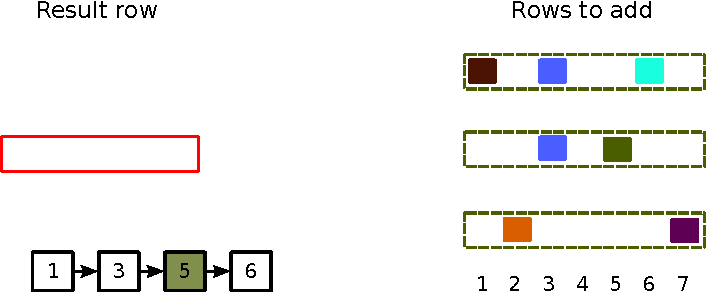
\includegraphics[width=0.7\textwidth]{figures/spgemm-scalable-6} }\only<6>{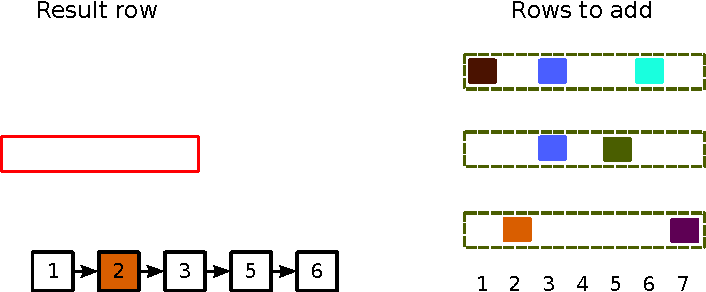
\includegraphics[width=0.7\textwidth]{figures/spgemm-scalable-7} }\only<7>{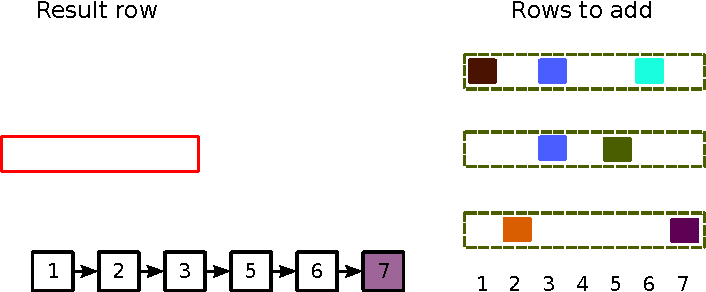
\includegraphics[width=0.7\textwidth]{figures/spgemm-scalable-8} }\only<8>{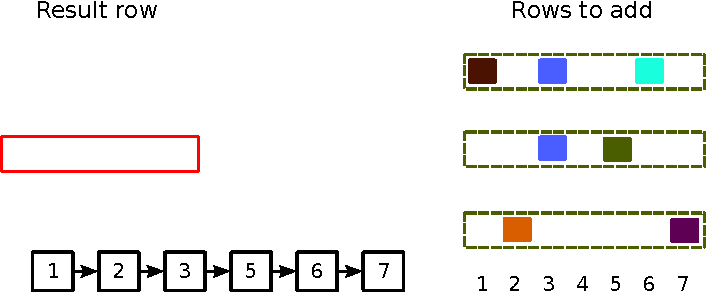
\includegraphics[width=0.7\textwidth]{figures/spgemm-scalable-9} }\only<9>{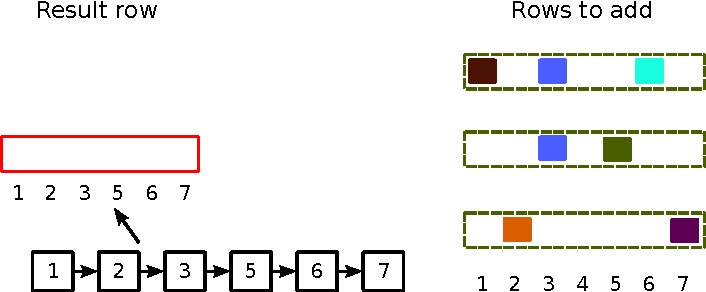
\includegraphics[width=0.7\textwidth]{figures/spgemm-scalable-10} }
\end{center}

 \begin{block}{Scalable MatMatMult in PETSc}
  \begin{itemize}
   \visible<2->{\item Use \{linked list, heap, binary tree\} to merge nonzero column indices}
   \visible<2->{\item No dense array}
  \end{itemize}
 \end{block}

\end{frame}

